\documentclass[12pt]{beamer}

% for themes, etc.
\mode<presentation>
{ \usetheme{Copenhagen}
  \usecolortheme{seahorse}{}
}
\setbeamertemplate{itemize items}[default]
\setbeamertemplate{enumerate items}[default]
\setbeamertemplate{navigation symbols}{}
\setbeamertemplate{headline}{}
\setbeamertemplate{footline}{}

\usepackage{times}  % fonts are up to you
\usepackage{proof}
\usepackage{listings}
\usepackage{courier}
\usepackage{graphicx}
\usepackage{stmaryrd}

\usepackage{tikz}
\newcommand*\circled[1]{\tikz[baseline=(char.base)]{
            \node[shape=circle,draw,double,inner sep=1pt] (char) {#1};}}

\lstset{columns=fullflexible}
\lstset{
  literate={->}{$\to$ }{1}
           {(->)}{$(\to)$ }{1}
           {=>}{$\Rightarrow$ }{1}
           {<-:}{$\Mapsfrom$ }{1}
           {:E}{$\in$ }{1}
           {forall}{$\forall$}{1}
           {(<+>)}{($\oplus$) }{1}
           {<+>}{$\oplus$ }{1}
           {<<*>>}{$\circled{$\star$}$ }{1}
           {<<map>>}{$\circled{\$}$ }{1}
           {(<<map>>)}{($\circled{\$}$) }{1}
           {(<<*>>)}{($\circled{$\star$}$) }{1}
           {Nat}{$\mathbb{N}$}{1}
           {Int}{$\mathbb{Z}$}{1}
           {[|}{$\llbracket$ }{1}
           {|]}{$\llbracket$ }{1},
  escapeinside=||,
  moredelim=**[is][\color{red}]{@}{@},
}
\lstset{language=Haskell}

% these will be used later in the title page
\title{Programming in Vinyl}
\author{Jon Sterling\\
    FOBO
}

\begin{document}

% this prints title, author etc. info from above
\begin{frame}
\titlepage
\end{frame}

\section{Extensible Records and Row Polymorphism}

\begin{frame}[fragile]
  \frametitle{Records in GHC 7.8}\pause
  \begin{itemize}
    \item Haskell records are nominally typed\pause
    \item They may not share field names
  \end{itemize}
  \pause
  \begin{lstlisting}
  data R = R { x :: X } |\pause|
  data R' = R' { x :: X } -- ^ Error
  \end{lstlisting}
\end{frame}

\begin{frame}
  \frametitle{Records in GHC 7.8}
  \only<1>{Records are...}
  \only<2>{\Large\centerline{anticompositional}}
\end{frame}

\begin{frame}
  \frametitle{Row Polymorphism}\pause
  How do we express the type of a function which adds a field to a record?\pause
  \only<3>{
    \[
      \infer{ f(x) : \{foo:A, bar:B\} }{ x : \{foo:A\} }
    \]
  }
  \only<4>{
    \[
      \infer{ f(x) : \{foo:A, bar:B; \vec{rs}\} }{ x : \{foo:A; \vec{rs}\} }
    \]
  }
\end{frame}

\begin{frame}
  \frametitle{Row Polymorphism}\pause
  \begin{itemize}
    \item supports type inference\pause
    \item is compositional\pause
  \end{itemize}
\end{frame}

\begin{frame}[fragile]
  \frametitle{Roll Your Own in Haskell}\pause
  \begin{lstlisting}
  data (s :: Symbol) ::: (t :: *) = Field |\pause|

  data Rec :: [*] -> * where |\pause|
    RNil :: Rec '[] |\pause|
    (:&) :: !t -> !(Rec rs) -> Rec ((s ::: t) ': rs)

  |\pause|
  class s :E (rs :: [*])|\pause|
  (=:) : s ::: t -> t -> Rec '[s ::: t]|\pause|
  (<+>) : Rec ss -> Rec ts -> Rec (ss ++ ts)
  \end{lstlisting}
\end{frame}

\begin{frame}[fragile]
  \frametitle{Roll Your Own in Haskell}\pause
  \begin{lstlisting}
  f :: (("a" ::: A :E rs) => Rec rs)
    -> (("a" ::: A :E rs, "b" ::: B :E rs) => Rec rs)
  \end{lstlisting}
\end{frame}

\section{Universes \`a la Tarski}

\begin{frame}
  \frametitle{Universes \`a la Tarski}\pause
  \begin{itemize}
    \item A type $\mathcal{U}$ of \textbf{codes} for types.
      \pause
    \item Function $\llbracket-\rrbracket_\mathcal{U} : \mathcal{U}\to\mathbf{Type}$.
      \pause
      \[
        \infer{
          \Gamma\vdash\llbracket s\rrbracket_\mathcal{U} : \mathbf{Type}
        }{
          \Gamma\vdash s : \mathcal{U}
        }
      \]
  \end{itemize}
\end{frame}

\begin{frame}
  \frametitle{Universes \`a la Tarski}
  \begin{center}
    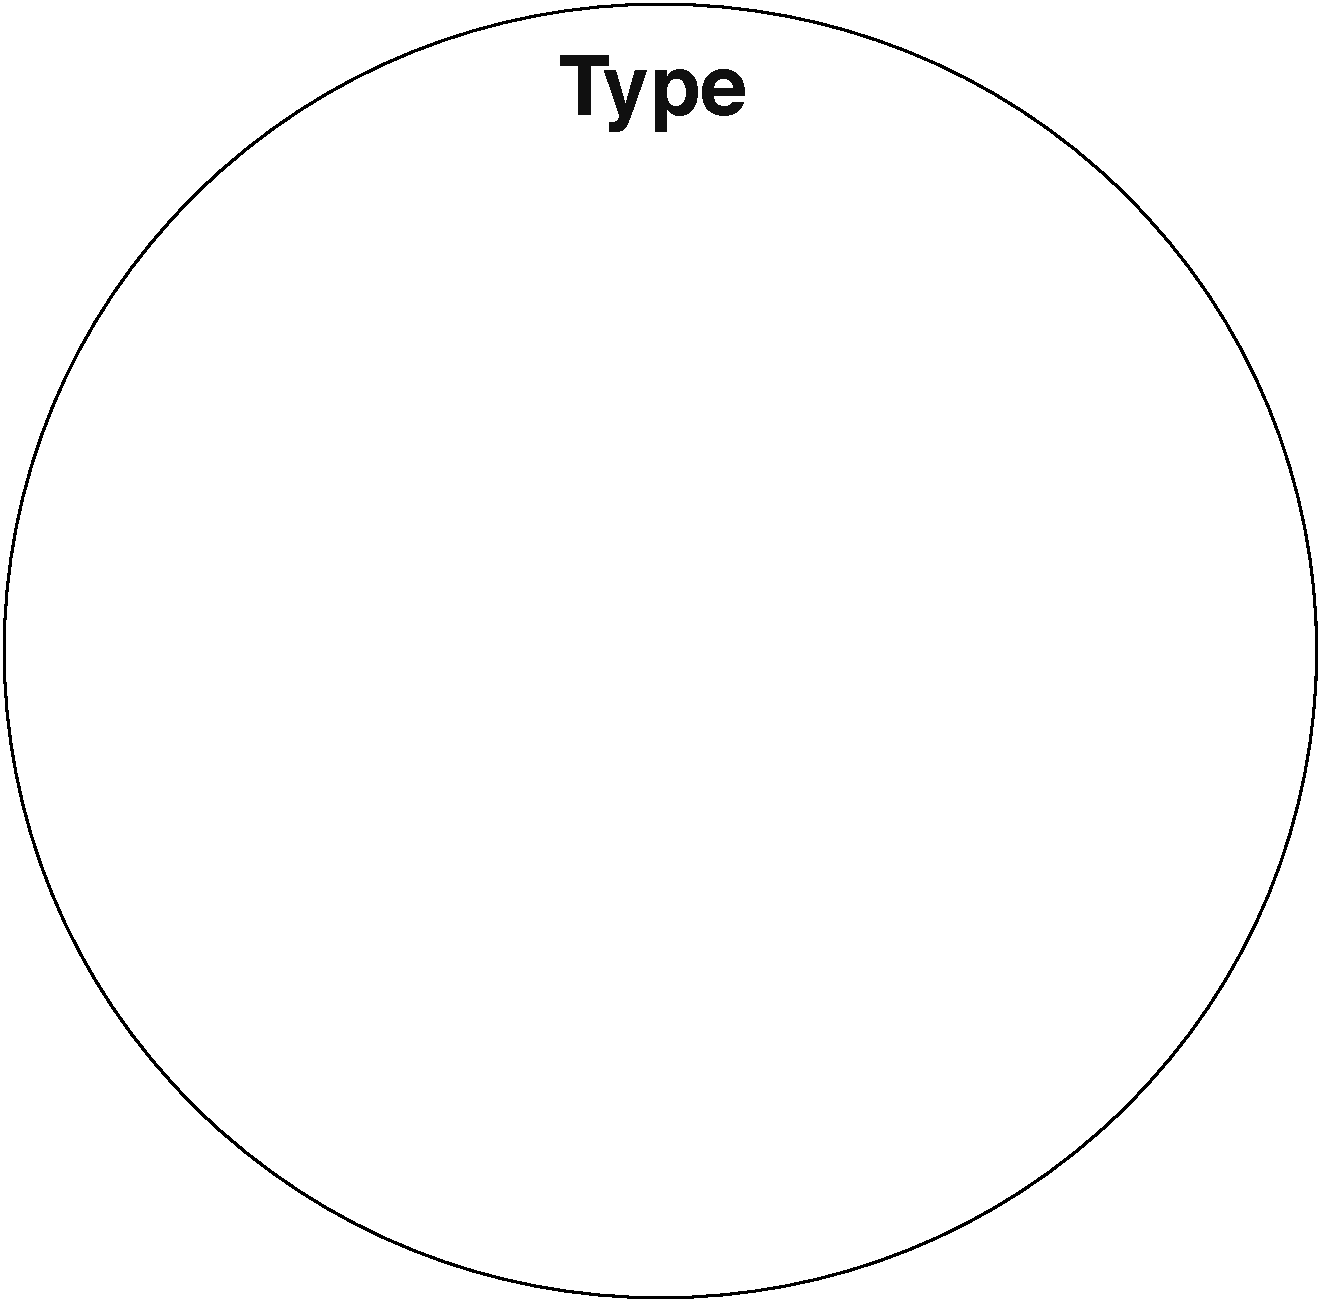
\includegraphics[width=2.8in]{universe-empty.pdf}
  \end{center}
\end{frame}

\begin{frame}
  \frametitle{Universes \`a la Tarski}
  \begin{center}
    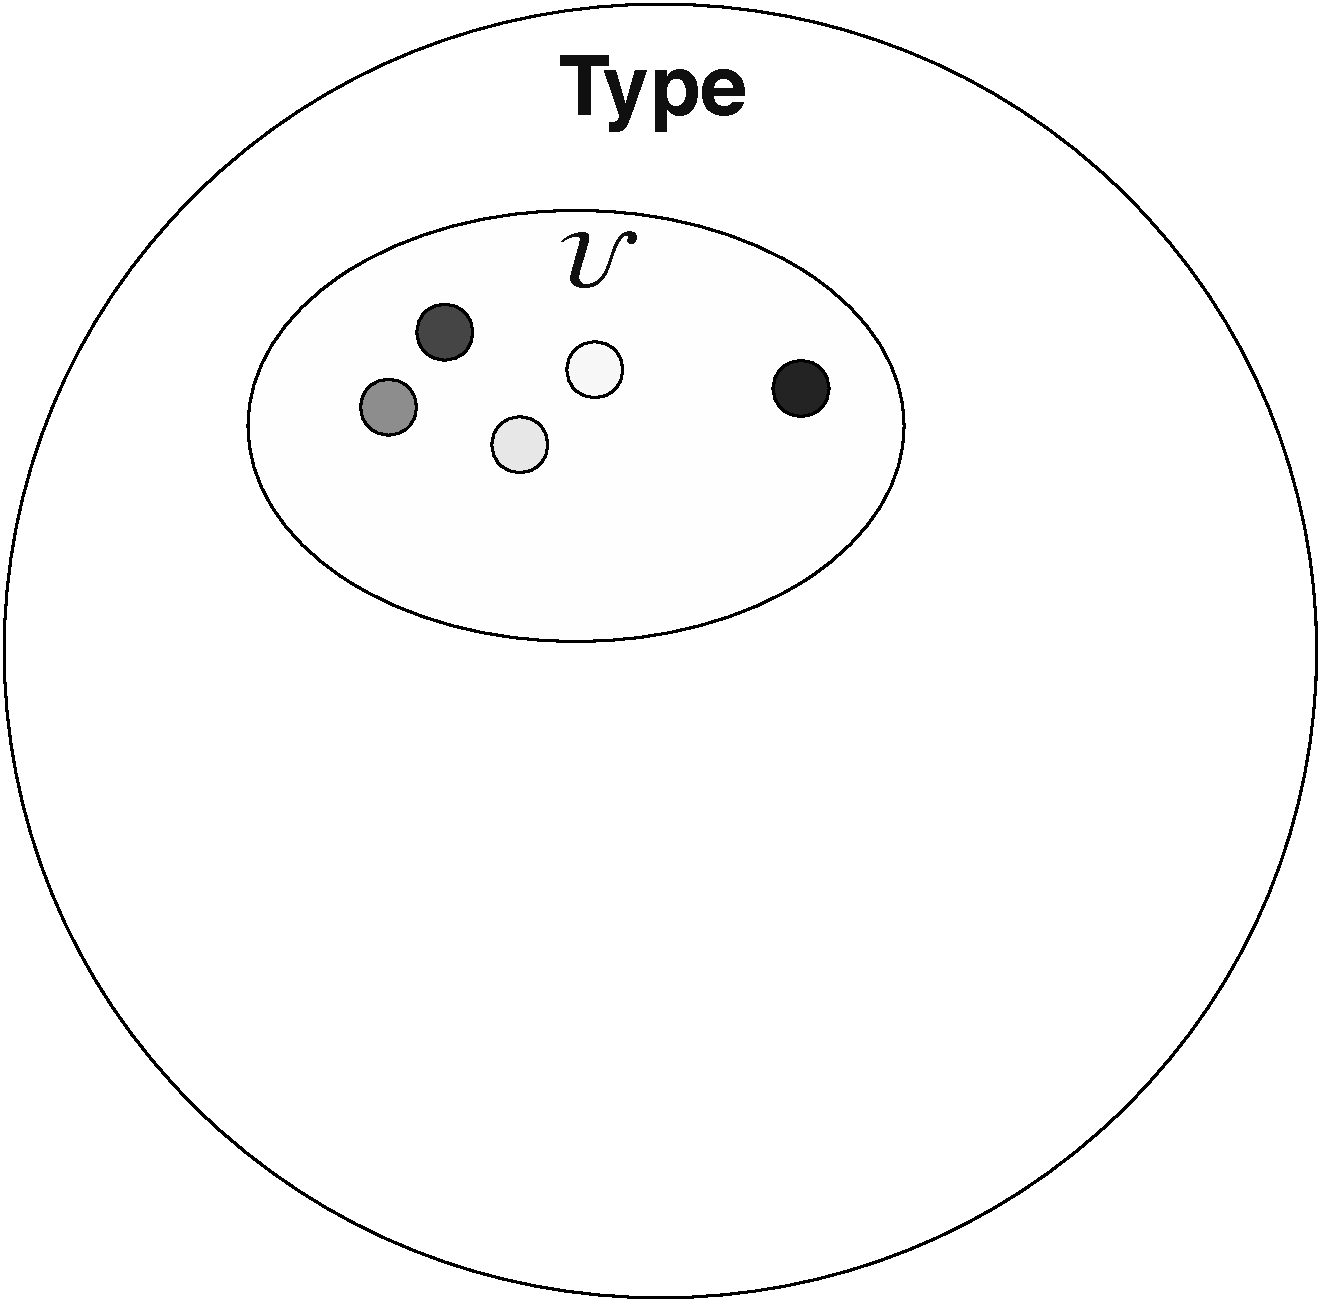
\includegraphics[width=2.8in]{universe-embedded.pdf}
  \end{center}
\end{frame}

\begin{frame}
  \frametitle{Universes \`a la Tarski}
  \begin{center}
    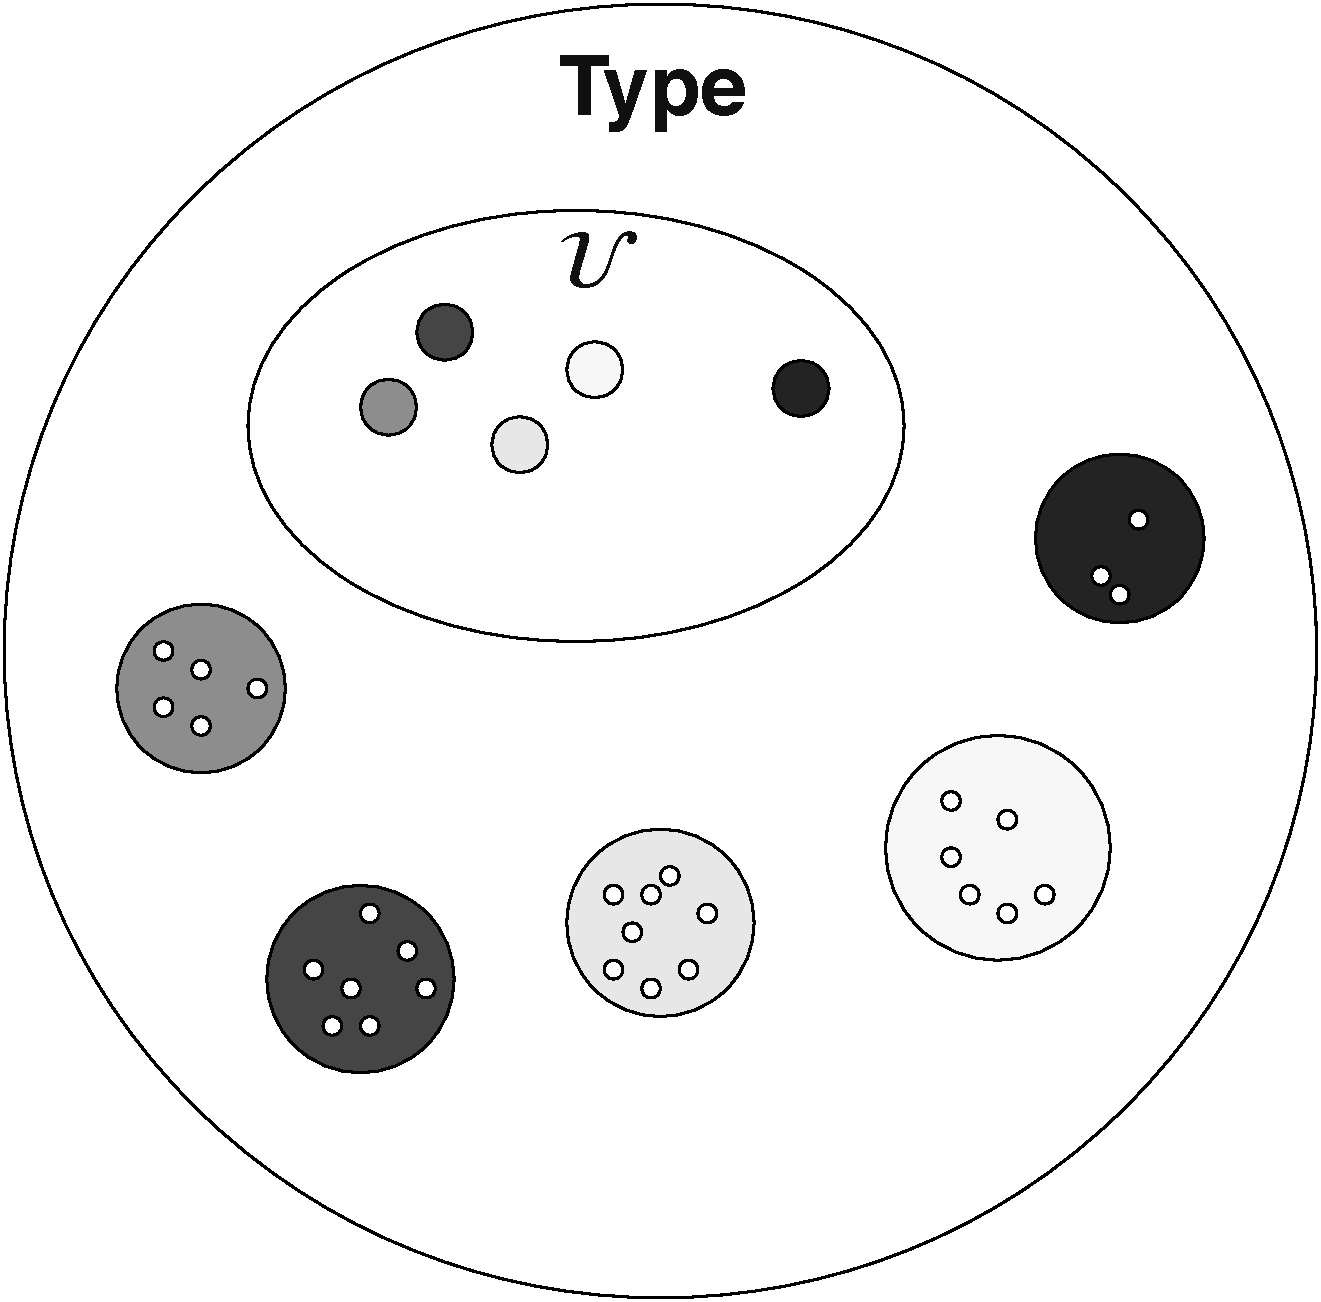
\includegraphics[width=2.8in]{universe-populated.pdf}
  \end{center}
\end{frame}

\begin{frame}
  \frametitle{Universes \`a la Tarski}
  \begin{center}
    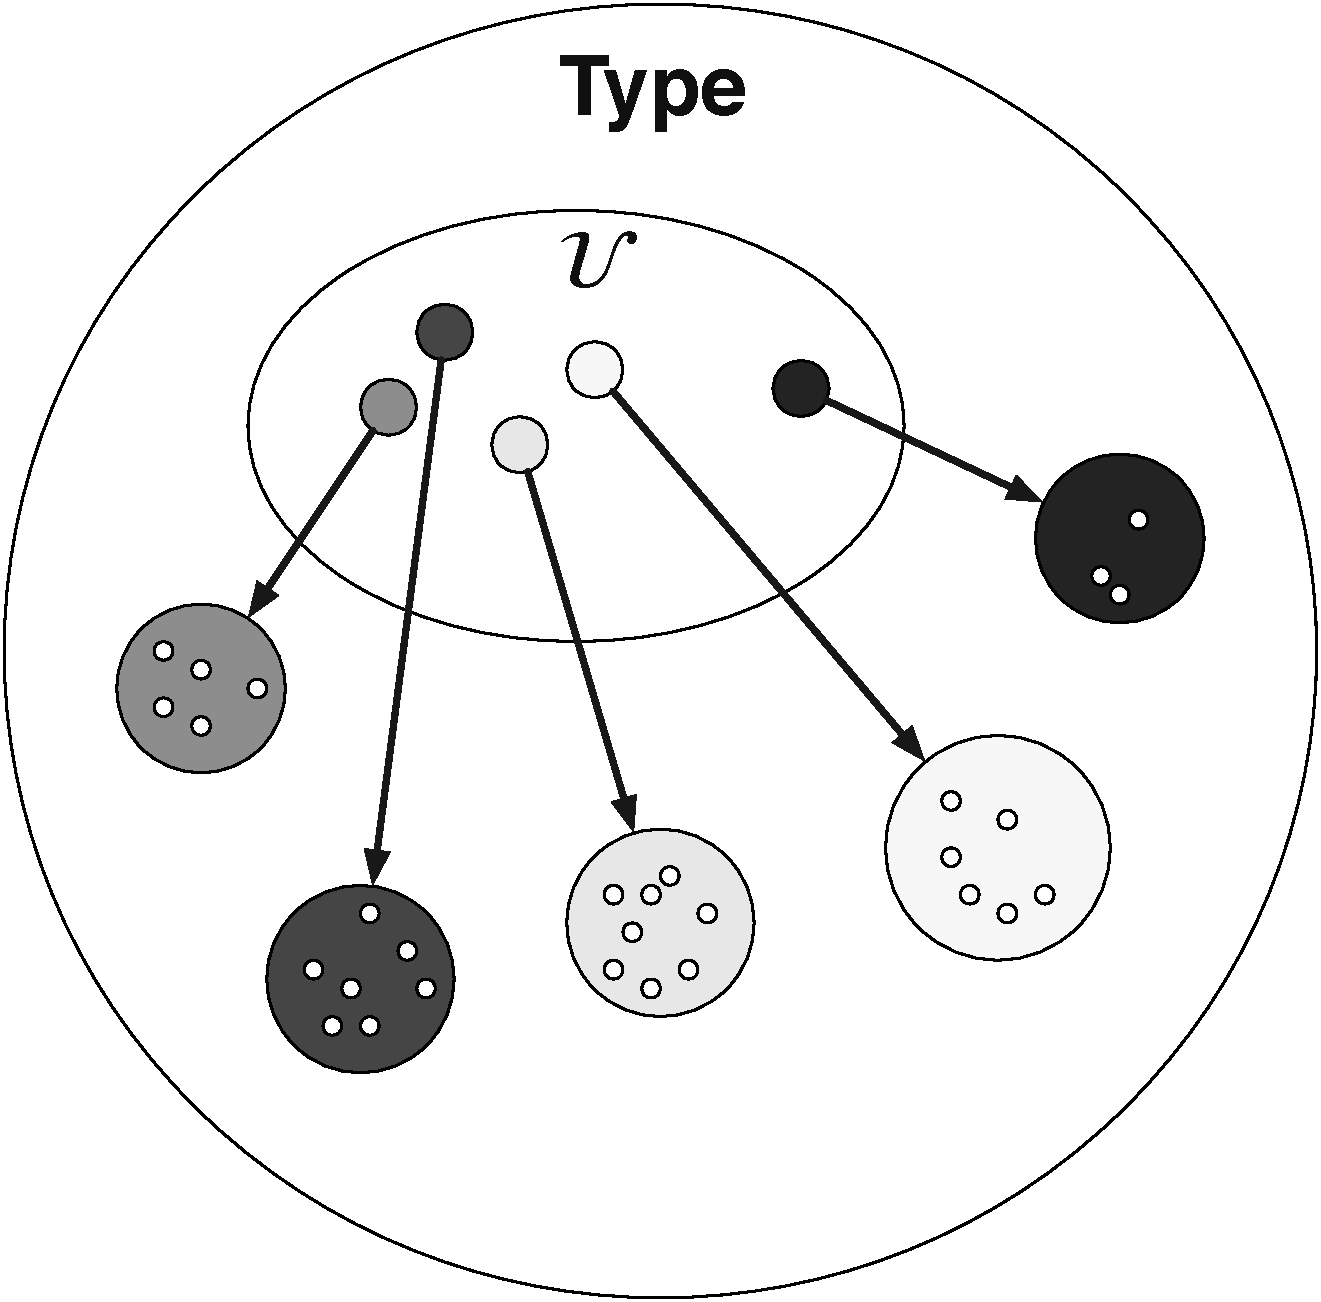
\includegraphics[width=2.8in]{universe-interpretation.pdf}
  \end{center}
\end{frame}

\begin{frame}
  \frametitle{A Closed Universe}
  \pause
  Let $\mathcal{A}$ be a universe of address books:
  \pause
  \begin{itemize}
    \item Statics:
      \pause
      \[
        \infer{\mathcal{A} : \mathbf{Type}}{}
        \qquad
        \pause
        \infer{\textsf{Label} : \mathbf{Type}}{}
        \qquad
        \pause
        \infer{\textit{Home}, \textit{Office} : \textsf{Label}}{}
      \]
      \pause
      \[
        \infer{\textsf{Name} : \mathcal{A}}{}
        \qquad
        \pause
        \infer{\textsf{Phone}[\ell],\textsf{Email}[\ell] : \mathcal{A}}{\ell : \textsf{Label}}
        \qquad
        \pause
        \infer{\llbracket s \rrbracket_\mathcal{A} : \mathbf{Type}}{s : \mathcal{A}}
      \]
      \pause
    \item Dynamics:
      \pause
      \[
        \infer{\llbracket \textsf{Name}\rrbracket_\mathcal{A} \leadsto \mathbf{string}}{}
        \qquad
        \pause
        \infer{\llbracket \textsf{Email}[\ell]\rrbracket_\mathcal{A} \leadsto \mathbf{string}}{}
      \]
      \pause
      \[
        \infer{\llbracket \textsf{Phone}[\ell]\rrbracket_\mathcal{A} \leadsto \mathbb{N}\;\mathbf{list}}{}
      \]
  \end{itemize}
\end{frame}


\section{Type-Theoretic Records}

\begin{frame}
  \frametitle{Records as Products}
  \pause
  \only<2,3>{
    Records: the product of the image of $\llbracket-\rrbracket_\mathcal{U}$ in $\mathbf{Type}$ restricted to a subset of the domain.
  }
  \only<4>{
    \begin{center}
      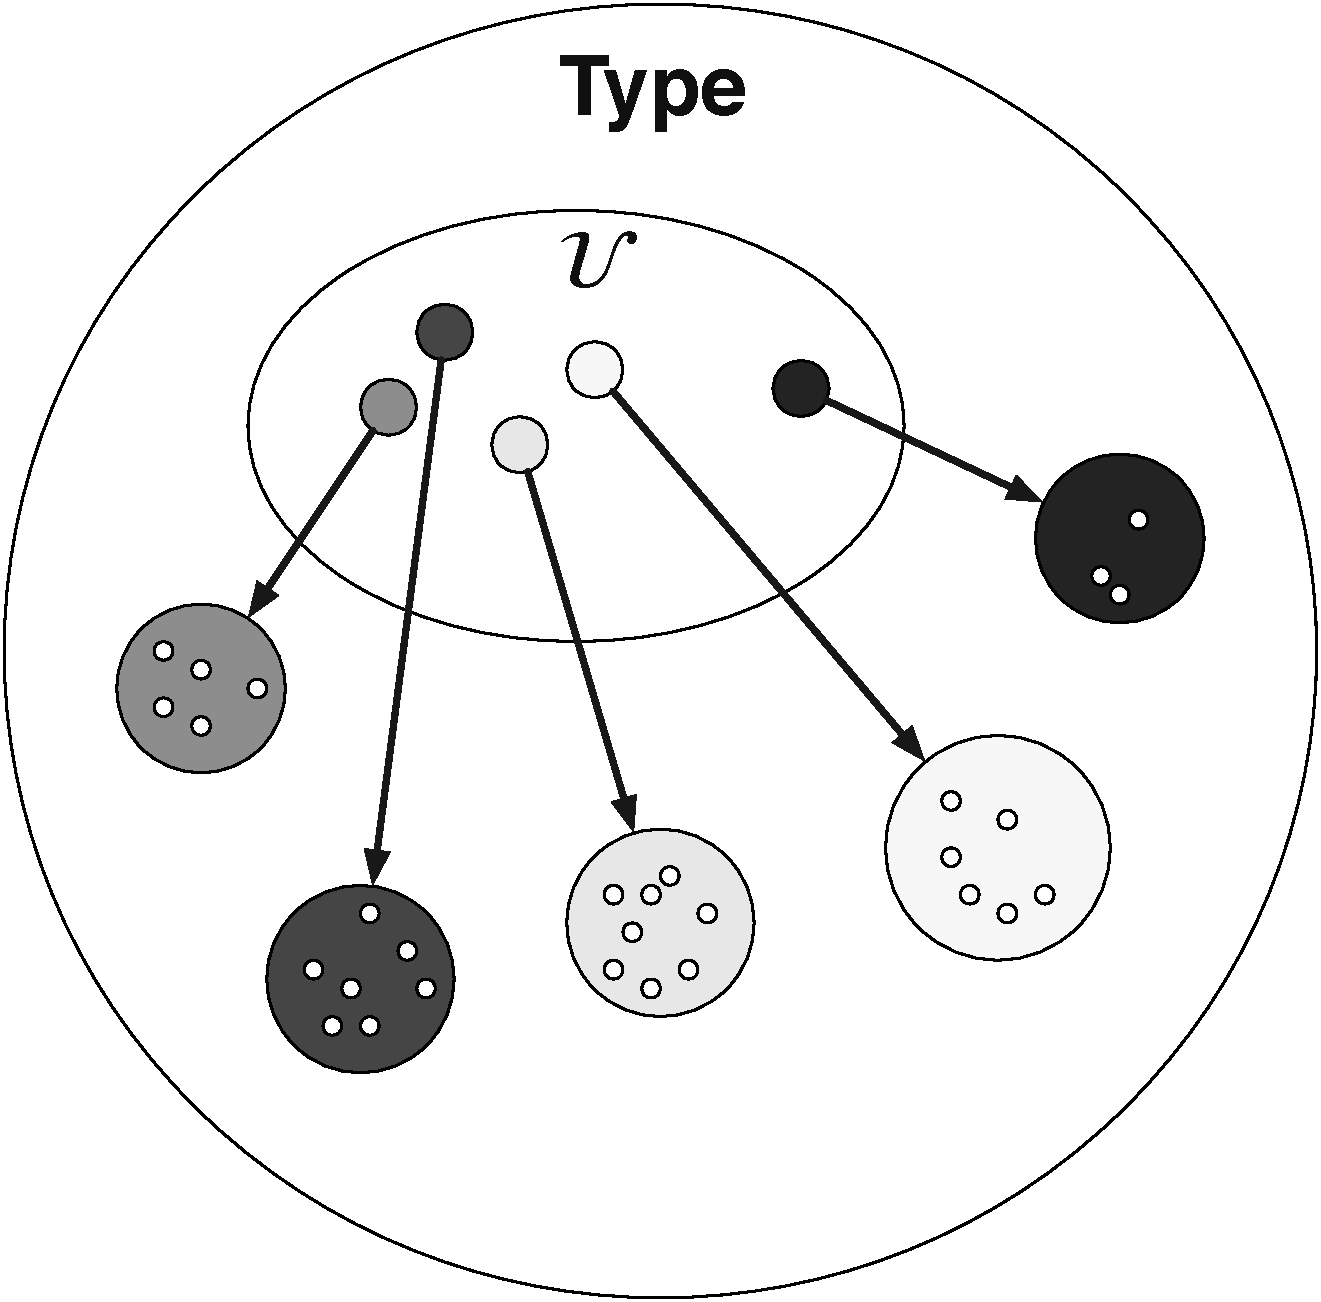
\includegraphics[width=2.8in]{universe-interpretation.pdf}
    \end{center}
  }
  \only<5>{
    \begin{center}
      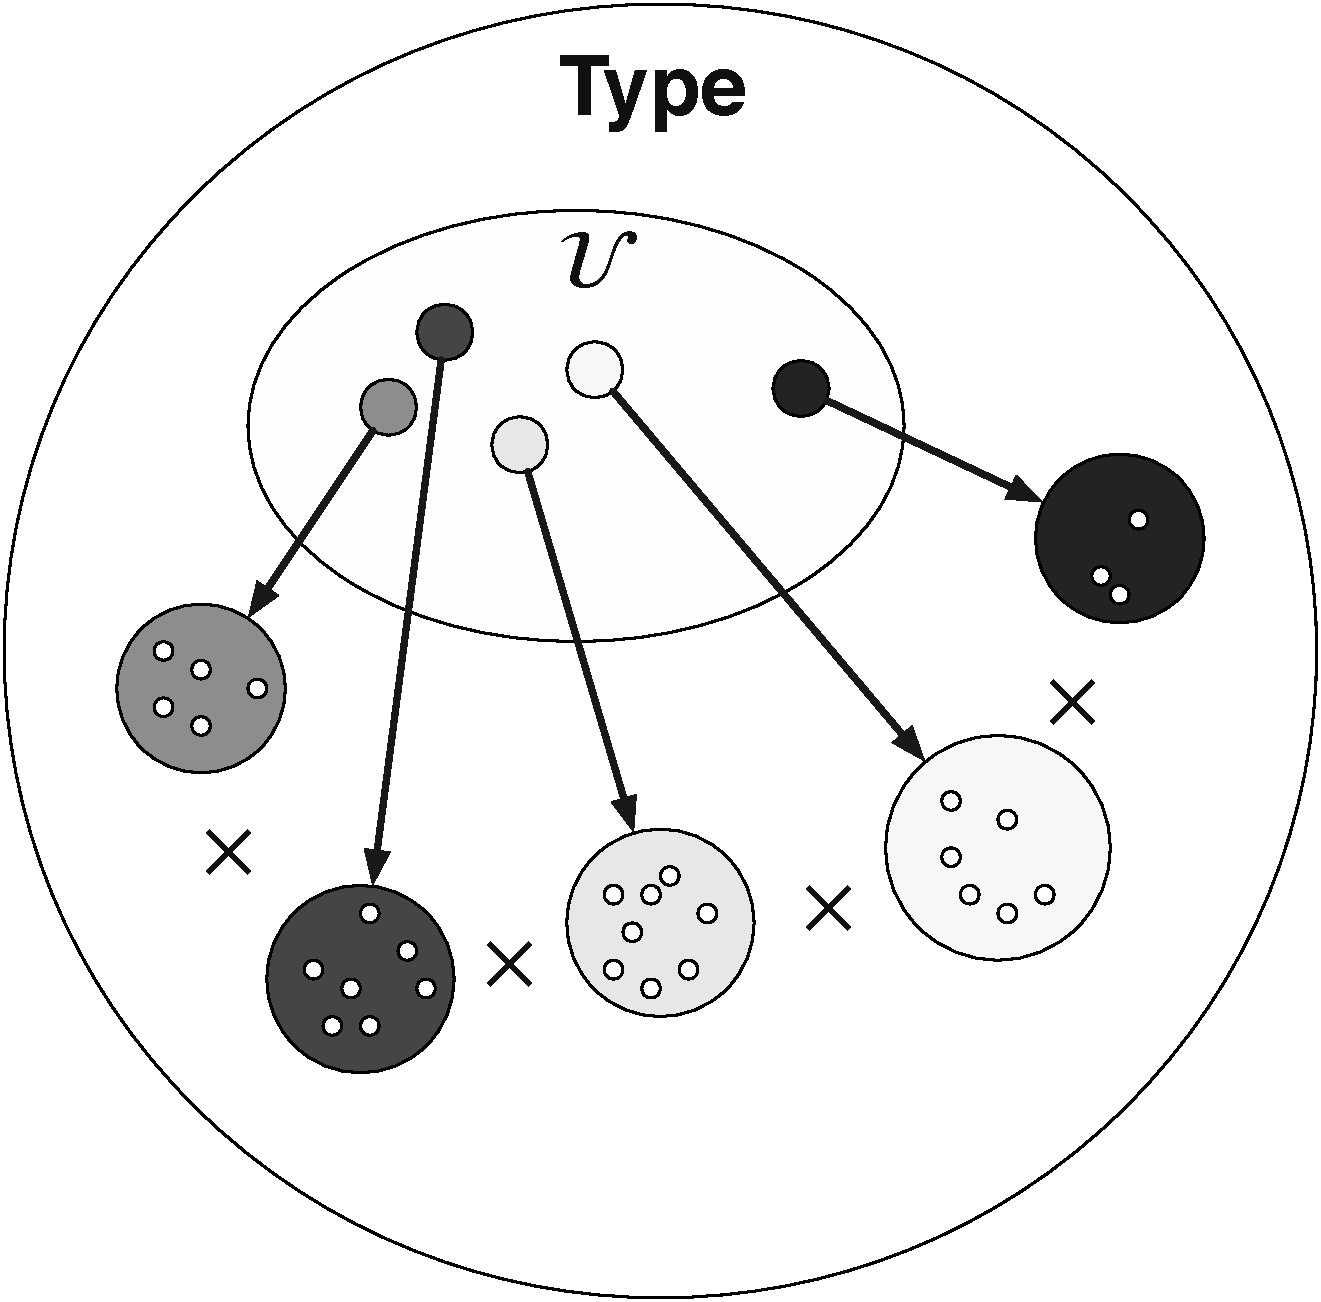
\includegraphics[width=2.8in]{universe-product.pdf}
    \end{center}
  }
  \only<3,6>{
    \[
      \mathsf{record}_\mathcal{U} \leadsto
        \sum_{\mathcal{V}:\mathbf{Type}}
        \sum_{i:\mathcal{V}\hookrightarrow\mathcal{U}}
        \prod_\mathcal{V} \llbracket-\rrbracket_\mathcal{U}\circ i
    \]
  }
\end{frame}

\begin{frame}
  \frametitle{Example Record}
  \[
    \begin{aligned}
      \mathsf{record}_\mathcal{U} &\leadsto
        \sum_{\mathcal{V}:\mathbf{Type}}
        \sum_{i:\mathcal{V}\hookrightarrow\mathcal{U}}
        \prod_\mathcal{V} \llbracket-\rrbracket_\mathcal{U}\circ i \\\\ \pause
      \mathcal{A}' &\leadsto \{ \mathsf{Name}, \mathsf{Email}\ \textit{Work} \}\\
      ex &: \mathsf{record}_\mathcal{U}\\ \pause
      ex &\leadsto \langle\mathcal{A}',\lambda x. x, \lambda.\\
         &\qquad \{\mathsf{Name}\mapsto \text{"Robert Harper"};\\
         &\qquad \ \mathsf{Email}\ \textit{Work}\mapsto \text{"rwh@cs.cmu.edu"} \}\rangle
    \end{aligned}
  \]
\end{frame}

\begin{frame}
  \frametitle{Corecords as Sums}
  \pause
  \only<2,3>{
    Corecords (extensible variants): the sum of the image of $\llbracket-\rrbracket_\mathcal{U}$ in $\mathbf{Type}$ restricted to a subset of the domain.
  }
  \only<4>{
    \begin{center}
      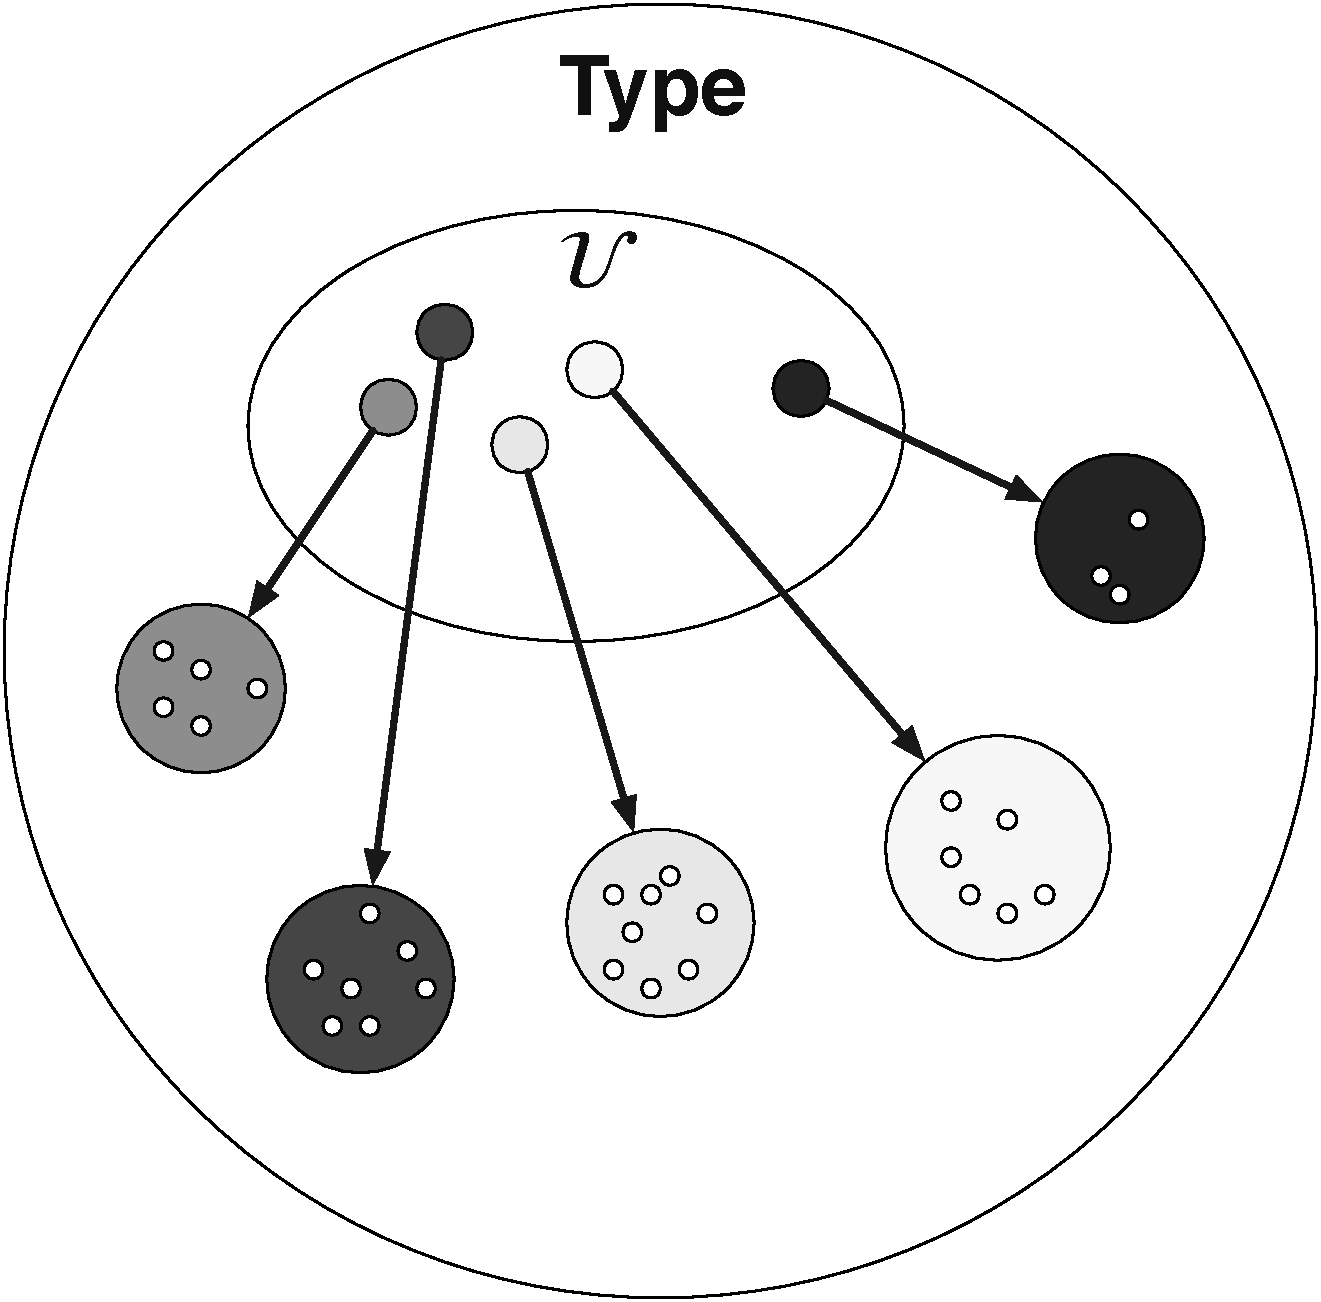
\includegraphics[width=2.8in]{universe-interpretation.pdf}
    \end{center}
  }
  \only<5>{
    \begin{center}
      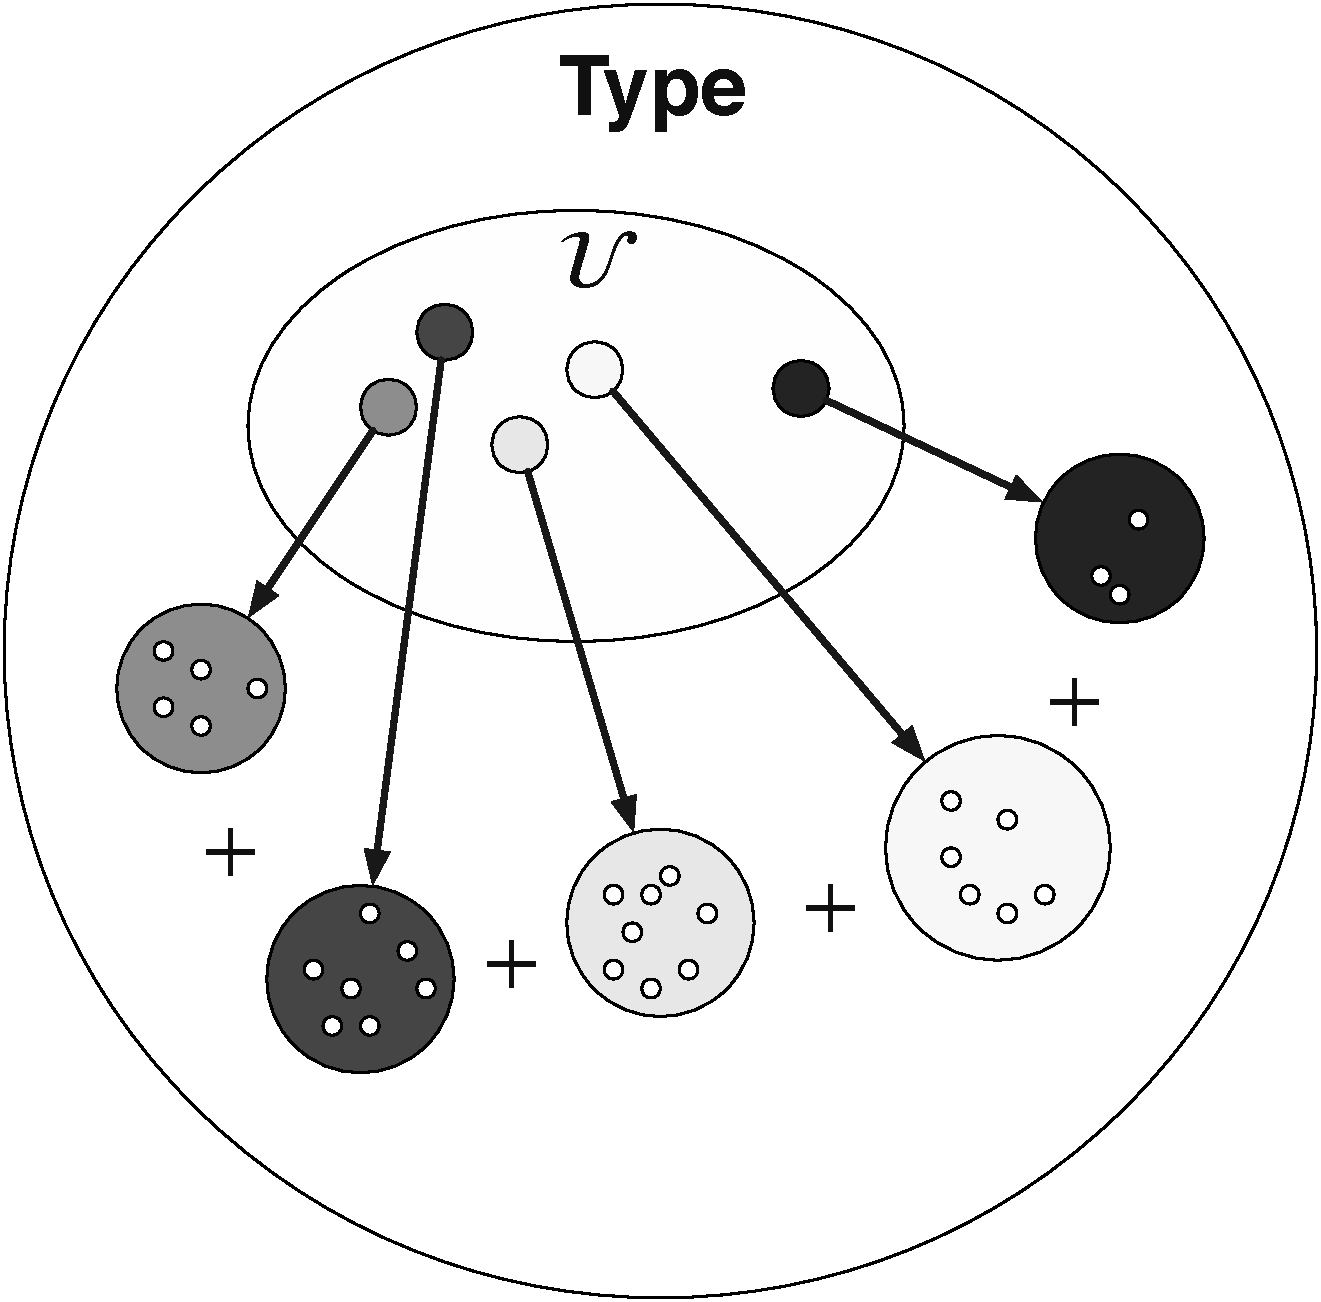
\includegraphics[width=2.8in]{universe-sum.pdf}
    \end{center}
  }
  \only<3,6>{
    \[
      \mathsf{corecord}_\mathcal{U} \leadsto
        \sum_{\mathcal{V}:\mathbf{Type}}
        \sum_{i:\mathcal{V}\hookrightarrow\mathcal{U}}
        \sum_\mathcal{V} \llbracket-\rrbracket_\mathcal{U}\circ i
    \]
  }
\end{frame}

\begin{frame}
  \frametitle{Doing it in Haskell}
  \pause
  \begin{itemize}
    \item Create a universe $\mathcal{U}$ at the type-level \pause
    \item Use type families to approximate $\llbracket-\rrbracket_\mathcal{U}$ \pause
    \item Parameterize \lstinline{Rec} by $\mathcal{U}$, $\llbracket-\rrbracket_\mathcal{U}$?
  \end{itemize}
\end{frame}

\begin{frame}[fragile]
  \frametitle{Records in Haskell}
  \begin{lstlisting}
  data Rec :: (|$\mathcal{U}$| -> *) -> [ |$\mathcal{U}$| ] -> * where |\pause|
    RNil :: Rec |$\llbracket-\rrbracket_\mathcal{U}$| '[] |\pause|
    (:&) :: !|$\llbracket$|r|$\rrbracket_\mathcal{U}$| -> !(Rec |$\llbracket-\rrbracket_\mathcal{U}$| rs) -> Rec |$\llbracket-\rrbracket_\mathcal{U}$| (r ': rs)
  \end{lstlisting}
\end{frame}

\begin{frame}[fragile]
  \frametitle{Recovering HList}\pause
  \begin{lstlisting}
  type HList rs = Rec (|$\Lambda\tau.\;\tau$|) rs|\pause|

  ex :: HList [Int, Bool, String] |\pause|
  ex = 34 :& True :& "vinyl" :& RNil
  \end{lstlisting}
\end{frame}

\section{Effectful Records}

\begin{frame}[fragile]
  \frametitle{Validating Records}

  \begin{lstlisting}
  bob :: Rec |$\llbracket-\rrbracket_\mathcal{A}$| [Name, Email Work] |\pause|
  bob = Name =: "Robert Harper"
      <+> Email Work =: "rwh@cs.cmu.edu"
  \end{lstlisting}
  \pause
  \begin{lstlisting}
  validateName :: String -> Either Error String
  validateEmail :: String -> Either Error String
  validatePhone :: [Nat] -> Either Error [Nat]
  \end{lstlisting}
  \pause
  \centerline{\textit{*unnnnnhhh...*}}
  \pause
  \begin{lstlisting}
  validateContact
    :: Rec |$\llbracket-\rrbracket_\mathcal{A}$| [Name, Email Work]
    -> Either Error (Rec |$\llbracket-\rrbracket_\mathcal{A}$| [Name, Email Work])
  \end{lstlisting}
\end{frame}
\begin{frame}
  \centerline{\textbf{Welp.}}
\end{frame}

\begin{frame}[fragile]
  \frametitle{Effects inside records}
  \begin{lstlisting}
  data Rec :: (|$\mathcal{U}$| -> *) -> [ |$\mathcal{U}$| ] -> * where
    RNil :: Rec |$\llbracket-\rrbracket_\mathcal{U}$| '[]
    (:&) :: !|$\llbracket$|r|$\rrbracket_\mathcal{U}$| -> !(Rec |$\llbracket-\rrbracket_\mathcal{U}$| rs) -> Rec |$\llbracket-\rrbracket_\mathcal{U}$| (r ': rs)
  \end{lstlisting}
\end{frame}
\begin{frame}[fragile]
  \frametitle{Effects inside records}
  \begin{lstlisting}
  data Rec :: (|$\mathcal{U}$| -> *) -> (* -> *) -> [ |$\mathcal{U}$| ] -> * where
    RNil :: Rec |$\llbracket-\rrbracket_\mathcal{U}$| f '[]
    (:&) :: !(f |$\llbracket$|r|$\rrbracket_\mathcal{U}$|) -> !(Rec |$\llbracket-\rrbracket_\mathcal{U}$| f rs) -> Rec |$\llbracket-\rrbracket_\mathcal{U}$| f (r ': rs)
  \end{lstlisting}
\end{frame}

\begin{frame}[fragile]
  \frametitle{Compositional Validation}

  \begin{lstlisting}
  type Rec|$_\mathcal{A}$| = Rec |$\llbracket-\rrbracket_\mathcal{A}$| |\pause|
  bob :: Rec|$_\mathcal{A}$| Identity [Name, Email Work] |\pause|
  bob = Name =: "Robert Harper"
      <+> Email Work =: "rwh@cs.cmu.edu"|\pause|
  \end{lstlisting}
\end{frame}

\begin{frame}[fragile]
  \frametitle{Compositional Validation}
  \begin{lstlisting}
  type Validator a = a -> Either Error a|\pause|
  validateName :: Rec|$_\mathcal{A}$| Validator '[Name]
  validatePhone :: forall |$\ell$|. Rec|$_\mathcal{A}$| Validator '[Phone |$\ell$|]
  validateEmail :: forall |$\ell$|. Rec|$_\mathcal{A}$| Validator '[Email |$\ell$|]|\pause|

  type TotalContact =
    [ Name, Email Home, Email Work
    , Phone Home, Phone Work ]|\pause|

  validateContact :: Rec|$_\mathcal{A}$| Validator TotalContact
  validateContact = validateName
                  <+> validateEmail
                  <+> validateEmail
                  <+> validatePhone
                  <+> validatePhone
  \end{lstlisting}
\end{frame}

\begin{frame}[fragile]
  \frametitle{Record Operators}\pause

  \begin{lstlisting}
  newtype Lift o f g x = Lift { runLift :: f x `o` g x }|\pause|

  type Validator = Lift (->) Identity (Either Error)|\pause|

  (<<*>>) :: Rec|$_\mathcal{U}$| (Lift (->) f g) rs -> Rec|$_\mathcal{U}$| f rs -> Rec|$_\mathcal{U}$| g rs|\pause|

  rdist :: Applicative f => Rec|$_\mathcal{U}$| f rs -> f (Rec|$_\mathcal{U}$| Identity rs)
  \end{lstlisting}
\end{frame}

\begin{frame}[fragile]
  \frametitle{Compositional Validation}

  \begin{lstlisting}
  newtype Lift o f g x = Lift { runLift :: f x `o` g x }
  type Validator = Lift (->) Identity (Either Error)
  (<<*>>) :: Rec|$_\mathcal{U}$| (Lift (->) f g) rs -> Rec|$_\mathcal{U}$| f rs -> Rec|$_\mathcal{U}$| g rs
  rdist :: Applicative f => Rec|$_\mathcal{U}$| f rs -> f (Rec|$_\mathcal{U}$| Identity rs)|\pause|

  validateContact :: Rec|$_\mathcal{A}$| Validator TotalContact|\pause|

  bobValid :: Rec|$_\mathcal{A}$| (Either Error) [Name, Email Work]|\pause|
  bobValid = cast validateContact <<*>> bob|\pause|

  validBob :: Either Error (Rec|$_\mathcal{A}$| Identity [Name, Email Work])|\pause|
  validBob = rdist bobValid
  \end{lstlisting}
\end{frame}

\begin{frame}
  \frametitle{Laziness as an effect}\pause

  \begin{itemize}
    \item Laziness considered harmful in the small\pause
    \item Vinyl records are strict in their constructors\pause
    \item Lazy variants usually accomplished through duplication\pause
    \item[$\uparrow$] \textbf{Utterly unacceptable}
  \end{itemize}
\end{frame}

\begin{frame}[fragile]
  \frametitle{Laziness as an effect}\pause

  \begin{lstlisting}
  newtype Identity a = Identity { runIdentity :: a }|\pause|
  data Thunk a = Thunk { unThunk :: a }|\pause|

  type PlainRec|$_\mathcal{U}$| rs = Rec|$_\mathcal{U}$| Identity rs|\pause|
  type LazyRec|$_\mathcal{U}$| rs = Rec|$_\mathcal{U}$| Thunk rs
  \end{lstlisting}
\end{frame}

\begin{frame}[fragile]
  \frametitle{Concurrent Records with Async}\pause

  \begin{lstlisting}
  fetchName :: Rec|$_\mathcal{A}$| IO '[Name]|\pause|
  fetchName = Name <-: someOperation|\pause|

  fetchWorkEmail :: Rec|$_\mathcal{A}$| IO '[Email Work]|\pause|
  fetchWorkEmail = Email Work <-: anotherOperation|\pause|

  fetchBob :: Rec|$_\mathcal{A}$| IO [Name, Email Work]|\pause|
  fetchBob = fetchName <+> fetchWorkEmail
  \end{lstlisting}
\end{frame}

\begin{frame}[fragile]
  \frametitle{Concurrent Records with Async}\pause

  \begin{lstlisting}
  newtype Concurrently a
    = Concurrently { runConcurrently :: IO a }|\pause|

  (<<map>>) :: (forall a. f a -> g a) -> Rec|$_\mathcal{U}$| f rs -> Rec|$_\mathcal{U}$| g rs|\pause|

  bobConcurrently :: Rec|$_\mathcal{A}$| Concurrently [Name, Email Work]|\pause|
  bobConcurrently = Concurrently <<map>> fetchBob|\pause|

  concurrentBob :: Concurrently (Rec|$_\mathcal{A}$| Identity [...])|\pause|
  concurrentBob = rdist bobConcurrently
  \end{lstlisting}
\end{frame}

\begin{frame}[fragile]
  \frametitle{Concurrent Records with Async}\pause

  \begin{lstlisting}
  fetchBob :: Rec|$_\mathcal{A}$| IO [Name, Email Work]
  bobConcurrently :: Rec|$_\mathcal{A}$| Concurrently [Name, Email Work]
  concurrentBob :: Concurrently (Rec|$_\mathcal{A}$| Identity [...])|\pause|

  bob :: IO (Rec|$_\mathcal{A}$| Identity [Name, Email Work])|\pause|
  bob = runConcurrently concurrentBob
  \end{lstlisting}
\end{frame}
\end{document}

